\documentclass{standalone}
\usepackage{tikz} \tikzset{inner sep=0pt, outer sep=0pt}
\begin{document}
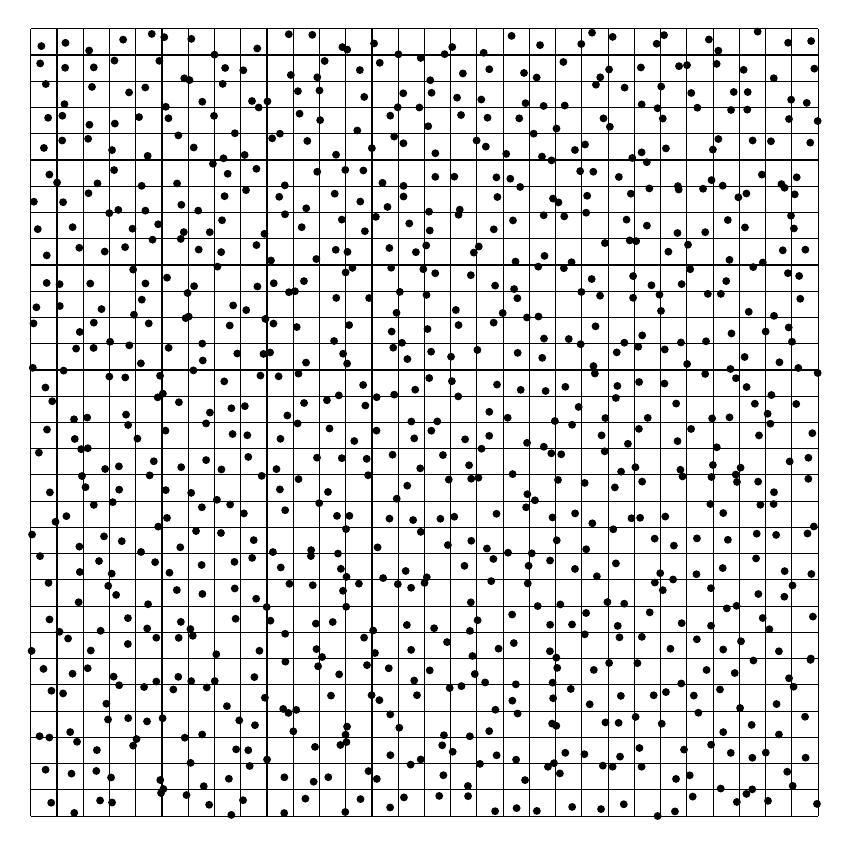
\begin{tikzpicture}
\draw[step=3.3333mm] (0,0) grid (100mm,100mm);
\foreach \x in {1,...,30} {
  \foreach \y in {1,...,30} {
    \pgfmathparse{3.3333*(rnd-1+\x)} \let\malx=\pgfmathresult
    \pgfmathparse{3.3333*(rnd-1+\y)} \let\maly=\pgfmathresult
    \node[xshift=\malx mm, yshift=\maly mm, circle, fill, minimum width=1mm]{};
  } % end of \foreach \y
} % end of \foreach \x
\end{tikzpicture}
\end{document}